\paragraph*{Objective} \hfill \\

\paragraph*{Results and procedure} \hfill\\
Using the Thevenin equivalent we find the smallest possible resistor for the output part, such that the current in the resistor remains less than 1mA, by:
\begin{align*}
R= \frac{V}{I} =\frac{16.1 V}{1mA} = 16.1k\Omega
\end{align*}
Now from the formula for power (P) we can derive that:
\begin{align*}
P&=\frac{V^2}{R} \,\,\,\,\, \text{for}&	R\rightarrow 0
\end{align*}
power (P) will be higher. 
The table that shows the power consumption for different resistances can be seen below.
\begin{table}[H]
	\centering
	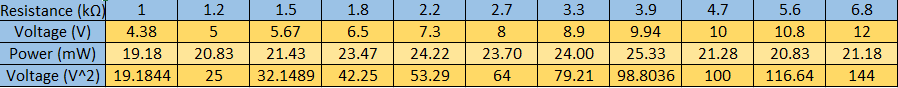
\includegraphics[width=1\textwidth]{./images/Kacper/23.png}
	\caption{Power consumption for different resistances}
	\label{Power consumption for different resistances}
\end{table}
\begin{flushleft}
Plot for the table(3) is drawn:
\end{flushleft}
\begin{figure}[H]
	\centering
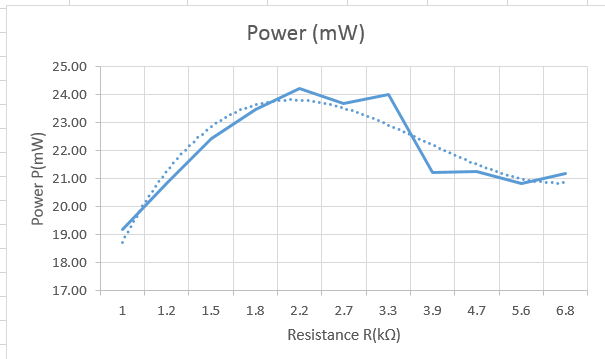
\includegraphics[width=1\textwidth]{./images/Kacper/23a.png}
	\caption{Power consumption}
	\label{Power consumption}
\end{figure}

\paragraph*{Conclusion} \hfill \\
We found out that the maximum power consumption is obtained when the resistance of the load matches the $R_{th}$, and falls when we increase the resistance of the load. 